% APS Open Science submission candidate for author review, 2026-10-28
\documentclass[%
  aps,physrev,onecolumn,10pt,amsmath,amssymb,superscriptaddress,longbibliography,floatfix
]{revtex4-2}

\usepackage{graphicx}
\usepackage{dcolumn}
\usepackage{bm}
\usepackage{physics}
\usepackage{hyperref}
\hypersetup{hidelinks,pdfauthor={Vinayak M. Kulkarni},pdftitle={Emergent PT Symmetry and Exceptional Points in a Driven Dirac Impurity}}
\pdfstringdefDisableCommands{\def\PT{PT}\def\({}\def\){}\def\tb{beta}\def\gb{beta0}}
\usepackage{xcolor}
\usepackage{booktabs}
\usepackage{enumitem}
\usepackage{placeins}

\newcommand{\PT}{\mathcal{PT}}
\newcommand{\Hss}{H_{\rm ss}}
\newcommand{\Htilde}{\tilde{H}}
\newcommand{\teps}{\tilde{\epsilon}_{\xi}}
\newcommand{\keff}{\kappa_{\rm imp}}
\newcommand{\Eep}{E_{\rm EP}}
\newcommand{\Gless}{G^{<}}
\newcommand{\Gret}{G^{R}}
\newcommand{\Gadv}{G^{A}}
\newcommand{\tb}{\tilde{\beta}}          % gauge-invariant SBMF scale
\newcommand{\gb}{\beta_0}               % signed frozen drive-control amplitude
\newcommand{\Gpt}{\Gamma_{\mathrm{PT}}}   % projected gain/loss channel
\newcommand{\dSig}{\delta_{\Sigma}}          % real one-body self-energy shift
\newcommand{\Deff}{\Delta_{\rm eff}}     % projected coherent splitting/flip
\newcommand{\Dzero}{\Delta_0}              % static coherent splitting in generic projection
\newcommand{\Dcoh}{\Delta_{\rm coh}}          % Kramers--Kronig coherent detuning
\newcommand{\Veff}{V_{\rm eff}}           % projected impurity-bath hybridization
\newcommand{\cV}{c_V}

\begin{document}

\title{Emergent \texorpdfstring{$\PT$}{PT} Symmetry and Exceptional Points
       in a Driven Dirac Impurity}

\author{Vinayak M.~Kulkarni}
\thanks{JNCASR is the author's doctoral affiliation; this work was carried out independently}
\email{vmkphysimath@gmail.com}
\affiliation{Theoretical Sciences Unit,
  Jawaharlal Nehru Centre for Advanced Scientific Research,
  Jakkur, Bangalore 560064, India}

\date{October 28, 2026}

\begin{abstract}
A stationary rotating drive tunes the coalescence of two decaying impurity
resonances in a Hermitian model with a finite-band radial spin--orbit-coupled
bath and remote auxiliary levels. The exact auxiliary rotation supplies
coherent spin-odd coupling and modifies the bath's SOC-induced relative
decay. Retaining the full frequency dependence and both open helicity cuts,
we establish the exceptional point (EP) numerically through a nonlinear
double zero, a rank-one inverse kernel and pole exchange. Retuning the
controls gives an EP family as SOC varies, with positive physical decay
rates. The result concerns the complete causal resonance problem; exact
parity--time symmetry is confined to a normalized constant-core benchmark.
Interactions are then added to the same microscopic model. An exact
finite-chain self-energy provides an approximate continuum embedding with
matching pole topology at two chain lengths in a nearly empty regime.
A continuum Kotliar--Ruckenstein saddle also admits EPs at and near mean
filling one, where substantial double occupancy identifies a
charge-fluctuating state. These results establish finite-chain and
mean-field continuations at their respective levels; a continuum-converged
local-moment EP remains unresolved.
\end{abstract}

\maketitle

% ============================================================
\section{Introduction}
\label{sec:intro}
% ============================================================

We ask whether a drive acting on remote bath orbitals can tune a
coalescence of decaying impurity resonances when finite-band dispersion and
the complete causal frequency dependence are retained. Driven impurities
connect this question to local interactions and state preparation.
Keldysh methods provide a framework for their response
~\cite{kamenev2023field,popruzhenko2014keldysh,maghrebi2016nonequilibrium};
related approaches address dissipative impurities and open spin
systems~\cite{kulkscipo,Claeys2022RGdissipative}.
Exceptional points (EPs), at which eigenvalues and eigenvectors coalesce,
have been studied in boundary-sensitive bands~\cite{YaoWang2018},
interacting atoms~\cite{higherorder}, dissipative Hubbard
models~\cite{PhysRevLett.126.110404}, and photonic, acoustic and diffusive
systems~\cite{xia2021nonlinear,smirnova2020nonlinear,xue2022topological,
RevModPhys.96.015002,dai2024non,PhysRevLett.132.156901,khanikaev2024topological}.
Condensed-matter observations are reported in
Ref.~\cite{li2024discoverynonhermitianphasetransition}.

For correlated electrons, lattice coherence~\cite{wan2023evidence},
driven exchange~\cite{mentink2015ultrafast}, nonequilibrium
DMFT~\cite{aoki2014nonequilibrium} and real-time impurity
solvers~\cite{PhysRevX.7.031013} motivate studying how a drive changes local
resonances.  Exactly solved boundary and impurity models
~\cite{kattel2024kondo,kattel2024spin,kattel2024dissipation},
non-Hermitian RG and causality studies
~\cite{PhysRevB.111.125157,han2023complex,PhysRevB.111.045124},
and NRG, cold-atom and slave-boson approaches
~\cite{burke2025non,PhysRevLett.121.203001,SBkeld} address complementary
interaction questions.  Floquet multichannel Kondo
couplings~\cite{quito2023floquet} and dissipative Luttinger
liquids~\cite{PhysRevB.108.155120} are distinct settings.

Other settings include complex-hybridization Kondo breakdown
~\cite{yamamoto2026complex}, exact high-bias and time-dependent impurity
limits~\cite{oguri2013highbias,pasnoori2025tdkondo}, and Hermitian equilibrium
$\PT$ protection in CeCo$_2$P$_2$~\cite{hu2025ceco2p2}.
A companion mathematical work~\cite{KulkarniYB2026} develops the controlled
linearized contact model; no integrability of the complete driven kernel is
claimed here.

Here we study a defined radial SOC bath with an impurity and driven remote
levels.  Its stationary rotating protocol produces a tunable coherent
spin-odd term that competes with the bath's SOC-induced relative decay.
The full-momentum result is an EP of two analytically continued impurity
resonance poles.  Exact $\PT$ symmetry is used only for a normalized
constant-core benchmark; it is not assumed for the full frequency-dependent
kernel.  The distinction also separates the retarded pole calculation from
the thermal closure used in supporting Keldysh checks.

Projection of a Hermitian system-plus-continuum Hamiltonian to a
non-Hermitian resonance problem, including impurity EPs, is
established~\cite{garmon2012analysis,garmon2021dynamics}.
Our contribution is the explicit connection between the stationary drive
and a family of passive resonance EPs in the specified finite-band bath.
The same bath determines the coherent coupling and relative decay, so the
double-zero and pole-exchange tests use its full analytic continuation.
This establishes the coalescence beyond the normalized constant-core
approximation and identifies the real controls needed to reach it.

The interaction calculations keep this stationary-drive Hamiltonian and
ask how the resonance pair continues after adding $U$. Exact finite-chain
responses supply a self-energy for an approximate continuum embedding;
a continuum slave-boson saddle independently tests filling and retuning
within mean field. The occupied saddle EP is charge fluctuating, so neither
mean filling one nor a large ratio $U/\bar\Gamma_0$ is identified with Kondo
strong coupling. Symmetry-protected interacting EPs are known in other
models~\cite{Schafer2022}; the separate spin-symmetric impurity control in
the Supplemental Material tests the role of symmetry without replacing
the SOC bath that generates the present mechanism.
Phenomenological non-Hermitian impurity and RG constructions address related
questions~\cite{PhysRevLett.121.203001,han2023complex,PhysRevB.111.045124}.
The normalized-core dynamics, thermal-closure checks and restricted contact
algebra help interpret the pole result; they are supporting analyses of
separately stated limits.

Figure~\ref{fig:overview} summarizes the model, the resonance EP and its
interaction continuations. Section~\ref{sec:model} defines the model.
Section~\ref{sec:coarse} contains the central causal-pole calculation and
finite-$U$ tests. Sections~\ref{sec:Hss}--\ref{sec:scattering} supply the
supporting effective-Hamiltonian, mean-field, response and scattering
analyses.

\begin{figure}[tb]
\centering
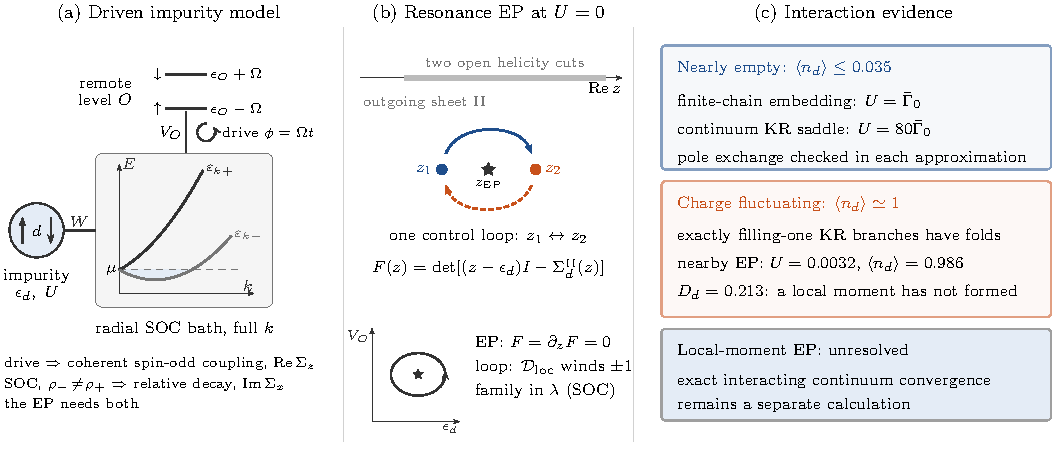
\includegraphics[width=\textwidth]{Fig0_overview.pdf}
\caption{\textbf{Model, pole EP and interaction evidence} (schematic).
(a) The impurity $d$ couples through $W$ to the full radial SOC bath, which
couples through $V_O$ to a remote fermionic level.  Uniform phase rotation
shifts the auxiliary energies by $\mp\Omega$.
(b) The outgoing-sheet inverse kernel has a rank-one double zero;
encircling it in two real controls exchanges the poles.
(c) The finite-chain embedding and continuum KR saddle give
method-specific interaction evidence.  Here $\bar\Gamma_0=W^2/4=0.0025$;
at $U=0$ the retarded EP is independent of filling.  The nearly occupied
KR points remain charge fluctuating, and their constrained folds do not
exclude nearby EPs.  This panel is not a phase diagram.}
\label{fig:overview}
\end{figure}

% ============================================================
\section{Model and Hamiltonian}
\label{sec:model}
% ============================================================

The Hermitian model is
$H=H_{\rm bath}+H_{\rm imp}+H_{\rm imp\text{-}bath}+H_O+H_{\rm hyb}[\phi(t)]$:
an Anderson impurity, a radial two-component bath, remote fermionic orbitals
and driven bath--orbital hoppings.  The linear-in-$k$ splitting motivates
``Dirac-like''; the quadratic curvature and cutoff are retained.
The Supplemental Material~\cite{suppmat} collects notation and parameters.

\subsection{Bath}

We define a radial effective bath, with the two-dimensional measure
$k\,dk/(2\pi)$ and fixed-axis SOC:
\begin{equation}
H_{\rm bath}
= \sum_{k,\sigma}\epsilon_k\,c^\dagger_{k\sigma}c_{k\sigma}
+ \lambda\sum_k k
  \bigl(c^\dagger_{k\uparrow}c_{k\downarrow}+\mathrm{h.c.}\bigr),
\label{eq:Hbath}
\end{equation}
where $c^\dagger_{k\sigma}$ creates a bath electron with radial
momentum $k$ (in units of inverse lattice constant) and spin
$\sigma\in\{\uparrow,\downarrow\}$;
$\epsilon_k=\alpha_{\rm b}k^2$ ($\alpha_{\rm b}>0$; $\alpha_{\rm b}=1$ in all
numerical calculations), with radial cutoff
$0\le k\le k_{\rm max}=\pi/4$; and $\lambda>0$ is the spin-orbit
coupling.  The separate energy cutoff $D_{\rm uv}$ enters only logarithmic
and scaling formulas below.
The SOC term in Eq.~(\ref{eq:Hbath}) uses one spin axis for every momentum
direction.  It is therefore odd under time reversal and is not the Rashba
coupling of a time-reversal-symmetric $C_{3v}$ host: for such a host and a
local $m=0$ orbital, $C_3$ forces the self-energy of the impurity spin
doublet to be diagonal, and no spin-mixing channel arises.
Equation~(\ref{eq:Hbath}) is accordingly an effective radial channel model.
An orbital impurity coupling to a suitable equal-$C_3$-character pair is one
possible realization to investigate; neither that construction nor a
host-specific projection is established here.
The chiral rotation $c_{k\pm}=(c_{k\uparrow}\pm c_{k\downarrow})/\sqrt{2}$
diagonalizes $H_{\rm bath}$ exactly, yielding SOC-split chiral
dispersions $\varepsilon_{k\pm}=\alpha_{\rm b}k^2\pm\lambda k$ with $\varepsilon_{k+}\neq\varepsilon_{k-}$ for all $k\neq0$.
For the full radial dispersions, the two positive-energy roots give
\begin{equation}
\begin{aligned}
\rho_+(\omega)&=\frac{\Delta-\lambda}{4\pi\alpha_{\rm b}\Delta},&
\rho_-(\omega)&=\frac{\Delta+\lambda}{4\pi\alpha_{\rm b}\Delta},\\
\Delta&=\sqrt{\lambda^2+4\alpha_{\rm b}\omega}.&&
\end{aligned}
\label{eq:exact_radial_dos}
\end{equation}
whenever both roots lie inside the radial cutoff.  Hence
$\rho_++\rho_-=1/(2\pi\alpha_{\rm b})$ for $\omega\to0^+$: the complete
quadratic-plus-SOC radial bath is not pseudogapped.  The familiar
$|\omega|/\lambda^2$ law describes only the small-$k$ cone patch of one
branch.  Below zero energy the lower branch instead has a band minimum at
$-\lambda^2/(4\alpha_{\rm b})$ and the associated radial van Hove edge.
The constant \emph{sum} makes the spin-even width flat, while the channel
difference $\rho_--\rho_+=\lambda/(2\pi\alpha_{\rm b}\Delta)$ remains; in the
full radial kernel this static difference, not the drive, supplies the
relative decay (Sec.~\ref{sec:coarse}).
The full-$k$ calculation below retains this exact structure; the symmetric
linear-DOS form is used only as an explicitly idealized analytic benchmark.

\subsection{Impurity}

The local Anderson impurity is $H_{\rm imp} =\sum_\sigma\epsilon_\xi\,d^\dagger_\sigma d_\sigma + U\,n_\uparrow n_\downarrow$,
where $d^\dagger_\sigma$ creates an impurity electron with spin
$\sigma$, $n_\sigma=d^\dagger_\sigma d_\sigma$ is the occupation,
$\epsilon_\xi$ is the bare impurity level before the projected
bath-induced detuning is included, and $U>0$ is the on-site Coulomb
repulsion.

\subsection{Impurity--Bath Hybridization}

The impurity couples directly to the $m=0$ (s-wave) bath channel via
\begin{equation}
H_{\rm imp\text{-}bath}
=\sum_{k,\sigma}
\left(W_k\,c^\dagger_{k,0,\sigma} d_\sigma + \mathrm{h.c.}\right),
\label{eq:Hcd}
\end{equation}
where $W_k$ is the bare hybridization amplitude.
$W_k$ is time independent and independent of the frozen drive control
$\beta_0$.  At the $U\to\infty$ slave-boson saddle the
physical spinon--bath vertex is $rW_k$, with $r=|b_c|$; in the finite-$U$
saddle of Sec.~\ref{sec:finiteU_KR} the scalar $r$ becomes a spin-dependent
matrix $R$.

The drive reaches the impurity only through the auxiliary dressing of this bath channel (Sec.~\ref{sec:coarse}).

\subsection{Auxiliary Angular-Momentum Modes}

As motivation for the auxiliary sector, a scalar trigonal term $\beta_3(k)k^3\cos3\theta$
(where $\beta_3(k)$ is the momentum-dependent trigonal crystal-field strength,
distinct from the hybridization amplitude $\gb$ introduced below;
and $\theta$ is the in-plane momentum angle) couples the
$m=0$ (s-wave) bath channel to higher angular-momentum harmonics $m=\pm3,\pm6,\ldots$ via the $C_3$ selection rule $\Delta m=\pm3$.
These higher harmonics are represented by auxiliary fermions
$O_{k,m,\sigma}$ with angular momentum index $m\neq0$:
\begin{equation}
\begin{split}
    H_O=\sum_{k,m\neq0,\sigma}
\epsilon_O^{(m)}\,&O^\dagger_{k,m,\sigma}O_{k,m,\sigma}\\
&+\sum_{\substack{k,m,\sigma\\m,m+3\ne0}}\beta_3(k)k^3
\bigl(O^\dagger_{k,m+3,\sigma}O_{k,m,\sigma}+\mathrm{h.c.}\bigr),
\label{eq:HO}
\end{split}
\end{equation}
where the mode energies satisfy $\epsilon_O^{(m)}=\epsilon_O^{(-m)}$
as a chosen symmetry of the auxiliary crystal-field sector.  This does not
restore time reversal of the fixed-axis bath.  The fields $O_{k,m,\sigma}$
provide remote off-shell levels ($\epsilon_O^{(m)}\gg D_{\rm uv}$) and are
integrated out exactly within the specified quadratic model.

\subsection{Periodic Drive and Hybridization}

The periodic drive couples the physical bath ($m=0$) to the remote
higher angular harmonics.  We write the Hermitian bath--auxiliary
hybridization as
\begin{equation}
H_{\rm hyb}[\phi(t)]
=\sum_{k,\sigma,m\neq0}
\bigl[
V_m(k)e^{i\zeta_\sigma\phi(t)}
c^\dagger_{k,0,\sigma}O_{k,m,\sigma}
+\mathrm{h.c.}\bigr] .
\label{eq:Hhyb}
\end{equation}
Here $\zeta_\uparrow=+1$ and $\zeta_\downarrow=-1$ label the spin projection,
and $V_m(k)$ is the chosen coupling from the radial channel to the
auxiliary sector, motivated by the scalar $C_3$ selection rule and
nonzero for $m=\pm3$ at this order; higher harmonics are reached through $H_O$.  An angle-resolved vertex $V_me^{i3m\theta}c^\dagger_{k,\theta,\sigma}$
would instead couple $O_m$ to the bath harmonic $3m\neq0$, which has no
overlap with the impurity channel.  The full-$k$ calculation keeps a single
remote level of this form, with vertex $V_O$ and energy $\epsilon_O$.  The normalized
frozen-kernel scans use the slow oscillatory protocol
$\phi(t)=(\pi/4)\sin(\Omega t)$.  In that protocol the passive
control is the instantaneous angular velocity
$\dot\phi(t_{\rm av})=(\pi\Omega/4)\cos(\Omega t_{\rm av})$; the numerical parameter
$\gb$ used below should be read as the corresponding effective
frozen-kernel amplitude, not as the value of the phase itself.  Hermiticity
fixes the second vertex to carry the complex-conjugate phase.  Therefore
the normal Gaussian contraction of a number-conserving auxiliary sector
contains phase differences, not phase sums.  This is important: the
off-shell auxiliary sector does not by itself generate anti-Hermitian
gain or loss.

The unitary change of variables
$O^{\rm lab}_{k,m,\sigma}=e^{-i\zeta_\sigma\phi(t)}
 O^{\rm rot}_{k,m,\sigma}$ removes the phase from Eq.~(\ref{eq:Hhyb}).
The vertices become phase-free and the auxiliary energies acquire the Berry
shift $\epsilon_O^{(m)}-\zeta_\sigma\dot\phi(t)$.
Thus a gapped Hermitian auxiliary sector produces a real spin-odd coherent
shift.  For the oscillatory protocol this statement is an adiabatic
low-energy projection.  For the stationary rotating protocol
$\phi(t)=\Omega t$, however, this energy shift is constant and
the rotated quadratic Hamiltonian is exactly time independent; no freezing
or gradient expansion in $\Omega$ is then required.  In this frame the drive
is equivalent to a static spin-dependent splitting $\mp\Omega$ of the remote
level, and its role is to make that splitting tunable.  Only the remote fields are rotated, so the conduction and impurity
operators are unchanged by this transformation.  Their occupations still
depend on the state preparation; a static Hamiltonian does not fix them.
The passive non-Hermitian component appears only in the second step, when
this shifted channel is embedded in the retarded Dirac bath.
For the oscillatory protocol the projection requires $|V|/\epsilon_O\ll1$ and
$\Omega\ll\epsilon_O$.  A full cycle sweeps the two signs of the frozen
control; nonadiabatic EP traversal and energy pumping are outside the scope
of this description.

% ============================================================
\section{Coarse Graining and Emergent \texorpdfstring{$\PT$}{PT} Symmetry}
\label{sec:coarse}
% ============================================================

\subsection{Keldysh Path Integral and Angular-Mode Integration}

We work within the Keldysh formalism~\cite{kamenev2023field}, writing
the partition function as a coherent-state path integral on the closed
time contour.  The bath and auxiliary angular modes enter quadratically
and can be eliminated at the Gaussian level.  The local Coulomb
interaction on the impurity is not treated in this Gaussian step; it is
treated below by self-energy embedding from exact finite-chain responses
(Sec.~\ref{sec:finiteU}) and by a finite-$U$ slave-boson saddle of the
continuum bath (Sec.~\ref{sec:finiteU_KR}).  The separate $U\to\infty$
slave-boson approximation in Sec.~\ref{sec:mf} is a supporting
constant-kernel benchmark.

Integrating out the auxiliary fields gives the influence kernel $\Xi_\sigma=V_\sigma g_OV_\sigma^\dagger$.  Because the auxiliary sector conserves particle number, the drive phases enter only as differences, and the Wigner transform shifts the auxiliary self-energy by $\zeta_\sigma\dot\phi$ (Supplemental Material).

To leading order in the slow drive and in the off-shell expansion, the
auxiliary-dressed $m=0$ bath therefore has the form $\Sigma_{\sigma}^{\rm bath,R}=\Sigma_0^{\rm bath,R}+\zeta_\sigma\Delta_{\rm aux}+O[(\Omega/\epsilon_O)^2]$.
Here $\Delta_{\rm aux}$ is real in the low-energy window.  Microscopically
one may write, schematically,
\begin{equation}
\begin{split}
\Delta_{\rm aux}(\omega,t_{\rm av})
=&-\dot\phi(t_{\rm av})\,\partial_{\epsilon_O}
\sum_{m\neq0}|V_m|^2 \\
&\times
\mathcal{P}\frac{1}{\omega-\epsilon_O^{(m)}} ,
\end{split}
\label{eq:Delta_aux}
\end{equation}
up to form-factor coefficients.

The bare impurity--bath hybridization $W_k$ in
Eq.~(\ref{eq:Hcd}) remains time independent.  The drive reaches the
impurity through the dressed bath propagator.  In contour notation the
two Gaussian eliminations give
\begin{align}
G_{c,\sigma}^{-1}
&=g_c^{-1}-\Xi_\sigma,
\qquad
\Xi_\sigma=V_\sigma\circ g_O\circ V_\sigma^\dagger,
\label{eq:dressed_c_inverse}\\
\Sigma_{d,\sigma}
&=W^\dagger\circ G_{c,\sigma}\circ W,
\label{eq:impurity_selfenergy_dressed_bath}
\end{align}
with $\circ$ the contour convolution; the drive enters only through the path $d\to c\to O\to c\to d$.

In the frozen off-shell window, write
$\Xi_\sigma^R=\Xi_0^R+\zeta_\sigma\delta\Xi^R$ with
$\delta\Xi^R\in\mathbb R$.  Expanding the dressed-bath resolvent gives the
general first-order correction
\begin{equation}
\delta\Sigma_d^R
=W^\dagger G_{c,0}^R\,\delta\Xi^R\,G_{c,0}^R W .
\label{eq:deltaSigma_exact}
\end{equation}
Although the auxiliary correction is real, the retarded continuum
propagators are complex, so the transmitted impurity correction has both
coherent and dissipative parts.  Defining $\Sigma_{d,0}^R(\omega)=\Lambda(\omega)-i\bar\Gamma(\omega)$,
we write $\Sigma^R_{d,\sigma} =\Sigma_{d,0}^R+\zeta_\sigma\Delta_{\rm coh} +i \zeta_\sigma\Gamma_{\rm PT}$.
For the nearly rigid scalar shift used in the analytic estimates,
$\delta\Xi^R\simeq\Delta_{\rm aux}$ and the spin-even auxiliary
background varies slowly.  Then
\begin{equation}
\Sigma^R_{d,\sigma}(\omega,t_{\rm av})
\simeq
\Sigma_{d,0}^R(\omega-\zeta_\sigma\Delta_{\rm aux})
\simeq
\Sigma_{d,0}^R-\zeta_\sigma\Delta_{\rm aux}
\partial_\omega\Sigma_{d,0}^R,
\label{eq:Dirac_conversion}
\end{equation}
which gives $\Delta_{\rm coh}=-\Delta_{\rm aux}\partial_\omega\Lambda$ and $\Gamma_{\rm PT}=\Delta_{\rm aux}\partial_\omega\bar\Gamma$.
Equation~(\ref{eq:deltaSigma_exact}) is the general first-order result;
Eq.~(\ref{eq:Dirac_conversion}) is its rigid-shift limit.  All functions
are evaluated in the active low-energy window.
For an SOC matrix bath, however, the exact result need not reduce to the
rigid shift of the spin-even scalar self-energy.  In the chiral basis set $a=(\omega^+-\varepsilon_{k+})^{-1}$,
$b=(\omega^+-\varepsilon_{k-})^{-1}$, so that
$g_0=(a+b)/2$ and $g_x=(a-b)/2$.  Then $-\partial_\omega g_0=g_0^2+g_x^2$ whereas $g_b\sigma_zg_b=(g_0^2-g_x^2)\sigma_z=ab\,\sigma_z$.
With the sign convention of Eq.~(\ref{eq:Delta_aux}), the exact first-order
relative coefficient is therefore
\begin{align}
\delta\Sigma_z^R
&=\Delta_{\rm aux}\sum_k|W_k|^2a_kb_k,
\notag\\
\Gamma_{\rm PT}
&=\Delta_{\rm aux}\!\left[
\partial_\omega\bar\Gamma
-2\,\operatorname{Im}\sum_k|W_k|^2g_{x,k}^2\right].
\label{eq:matrix_gamma_pt}
\end{align}
Reversing the definition of the spin-odd auxiliary shift reverses both sides
of Eq.~(\ref{eq:matrix_gamma_pt}), without changing any rate eigenvalue.
Two limits must be distinguished.  For a scalar energy-dependent width
($\partial_\omega\bar\Gamma\neq0$, $g_x=0$), Eq.~(\ref{eq:matrix_gamma_pt})
reduces to the rigid-shift result following Eq.~(\ref{eq:Dirac_conversion}) and the drive
generates a relative decay.  For the quadratic radial dispersion with constant $W_k=W$ and both
helicity roots open, both branches have radial velocity $\Delta$, so
$\operatorname{Im}\sum_k|W_k|^2a_kb_k=0$: the total width is flat,
$\operatorname{Im}\sum_k|W_k|^2g_{x,k}^2$ vanishes as well, and the
first-order relative decay is zero.  The cancellation holds to all orders in
the drive while both channels are open (Supplemental Material).  In the
full-$k$ kernel the drive therefore enters as a coherent spin-odd coupling,
and the relative decay originates in the SOC helicity imbalance
$\gamma=W^2\lambda/(4\alpha_{\rm b}\Delta)=\pi W^2(\rho_--\rho_+)/2$ at zero
drive.  Auxiliary dressing also changes the spin-mixing decay through the
on-shell roots; the cancellation of the spin-odd decay does not mean that
all dissipative coefficients are drive independent.

\subsection{Passive \texorpdfstring{$\PT$}{PT} Core and Causal Detuning}
\label{sec:PT_all}

The projected impurity self-energy is decomposed into a common bath part,
a passive relative decay imbalance, and a Kramers--Kronig-related coherent
detuning: $\Sigma_{\rm imp}^{R}=(\Lambda-i\bar\Gamma)\mathbb I+(\Dcoh+i\Gamma_{\rm PT})\sigma_z$.
The scalar term is a common Lamb shift and common decay.  It is retained in
the bath-controlled FDR, but at a fixed frequency it shifts both matrix eigenvalues equally.
Its frequency dependence is retained when locating resonance poles.
The spin-odd terms have different symmetry status:
$i\Gamma_{\rm PT}\sigma_z$ is the passive relative decay imbalance, while
$\Dcoh\sigma_z$ is a real coherent detuning generated by the same causal
retarded bath self-energy.

The SOC bath supplies the spin-mixing channel: a Hermitian principal-value
part and, through the helicity imbalance, an anti-Hermitian part.  In the original
spin basis, the local bath Green function has the matrix structure $g_b^R=[\omega^+-\epsilon_k-\lambda k\sigma_x]^{-1}=g_0\mathbb I+g_x\sigma_x$,
with $g_x(k,\omega)= \frac{\lambda k} {(\omega^+-\epsilon_k)^2-\lambda^2 k^2}$.
Equivalently, $g_x=(a-b)/2$ with the two chiral propagators defined above,
and the channel-odd self-energy is
\begin{equation}
\Sigma_x=\tfrac12(\Sigma_+-\Sigma_-)
=\tfrac12(\Lambda_+-\Lambda_-)-\tfrac{i}{2}(\Gamma_+-\Gamma_-).
\label{eq:complex_channel_odd_self_energy}
\end{equation}
The principal-value part of this SOC off-diagonal bath dressing gives a
real coherent spin-mixing coefficient, $\Deff(\omega)= \sum_k |W_k|^2\, {\rm Re}\, g_x(k,\omega)$,
renormalized in the interacting problem by the slave-boson saddle point.

The drive-induced shift cannot leak into this mixing channel at leading
order: expanding the dressed bath propagator to first order in the
spin-odd shift $\Delta_{\rm aux}\sigma_z$ gives $g_b^R\,\sigma_z\,g_b^R=\left(g_0^2-g_x^2\right)\sigma_z$,
because $\{\sigma_x,\sigma_z\}=0$.
For the scalar-shift benchmark, omitting the additional SOC loss imbalance
and subtracting the common damping defines the relative kernel
\begin{equation}
h_{\rm rel}=
\Deff\sigma_x+
\left(\Dcoh+i\Gamma_{\rm PT}\right)\sigma_z .
\label{eq:relative_detuned_kernel}
\end{equation}
The passive-$\PT$-symmetric core is obtained at the compensated detuning
point $\Dcoh=0$:
\begin{equation}
h_{\PT}=
\Deff\sigma_x+i\Gamma_{\rm PT}\sigma_z,
\qquad
\sigma_x h_{\PT}^*\sigma_x=h_{\PT} .
\label{eq:passive_PT_core}
\end{equation}
The real term $\Dcoh\sigma_z$ is not discarded.  It is $\PT$-odd under the
same operation and therefore acts as a causal detuning floor.  Exact $\PT$
symmetry with $P=\sigma_x$ is a property of this normalized core.  The
complete kernel also contains the imaginary spin-mixing part
$-i(\Gamma_+-\Gamma_-)\sigma_x/2$ of
Eq.~(\ref{eq:complex_channel_odd_self_energy}), which is $\PT$-odd under
$P=\sigma_x$.  In the exact radial kernel, where $\Gamma_{\rm PT}=0$, the roles
are exchanged: the leading-order dimer is $\Dcoh\sigma_z+i\gamma\sigma_x$ with
$\gamma=(\Gamma_--\Gamma_+)/2$, which is $\PT$-symmetric with $P=\sigma_z$, and
the real part of $\Sigma_x$ plays the role of the detuning in
Eq.~(\ref{eq:detuned_EP_conditions}) below.  The certified pole EP is the
nonlinear-pole version of this coalescence and does not rely on exact $\PT$
symmetry.  The squared half-splitting of the frozen matrix
Eq.~(\ref{eq:relative_detuned_kernel}) is $s^2= \Deff^2+ \left(\Dcoh+i\Gamma_{\rm PT}\right)^2$.
For real $\Deff$, $\Dcoh$, and $\Gamma_{\rm PT}$, exact coalescence in the
passive sector requires
\begin{equation}
\Dcoh\Gamma_{\rm PT}=0,
\qquad
\Deff^2+\Dcoh^2-\Gamma_{\rm PT}^2=0 .
\label{eq:detuned_EP_conditions}
\end{equation}
Thus, for a nonzero relative decay imbalance, the exact passive EP occurs
at the compensated point $\Dcoh=0$ and $|\Deff|=|\Gamma_{\rm PT}|$.
  Away from the
compensated point, the Kramers--Kronig detuning prevents a literal pole
coalescence.  Minimizing $|s|$ over real $\Deff$ at fixed $\Dcoh$ and $\Gamma_{\rm PT}$ gives $|s|_{\min}=\sqrt{2|\Dcoh\Gamma_{\rm PT}|}$
when $|\Dcoh|\leq|\Gamma_{\rm PT}|$; otherwise the minimum occurs at $\Deff=0$ and equals $\sqrt{\Dcoh^2+\Gamma_{\rm PT}^2}$.
For the idealized sharp-cutoff benchmark the floor is already
$0.90$--$1.00\,\Gamma_{\rm PT}$ one linewidth from the compensation energy,
so this frozen finite-band benchmark shows avoided coalescence
(Supplemental Material).

The rigid-shift estimate gives $\Gamma_{\rm PT}\sim\Omega|V|^2\epsilon_O^{-2}\partial_\omega\bar\Gamma$; reaching the normalized benchmark ratio $\Gamma_{\rm PT}/\bar\Gamma=0.10/0.12$ would require $\Omega/\epsilon_O\gtrsim1.061(\epsilon_O/|V|)^2$, incompatible with an off-shell quasistatic drive.  Supplemental Fig.~S1 therefore displays the constant-core geometry only.

\subsection{Stationary rotating-drive resonance EP}
\label{sec:causal_ep}
The preceding negative statement is specific to the normalized benchmark
and the oscillatory quasistatic protocol.  For $\phi(t)=\Omega t$, the
rotating-frame auxiliary levels are shifted by the constant $\mp\Omega$.
Keeping their exact frequency dependence, the curved SOC dispersion, and
the complete radial momentum integral, define on the outgoing resonance
sheet
\begin{equation}
F(z;\epsilon_d,V_O)=
\det\!\left[(z-\epsilon_d)\mathbb I-
\Sigma_d^{\mathrm{II}}(z;V_O)\right] .
\label{eq:full_k_pole_determinant}
\end{equation}
Here $z$ is complex energy, $\epsilon_d$ denotes the bare impurity gate in
this full-bath calculation, and II labels the outgoing resonance sheet
(SM App.~B).  A nonlinear pole EP is a double zero
$F=\partial_zF=0$ with $\partial_z^2F\neq0$ and a rank-one inverse kernel.
To certify its existence without evaluating a singular eigenbasis, let
$z_c(\epsilon_d,V_O)$ be the continuously branch-tracked solution of
$\partial_zF(z_c)=0$ on a closed control loop $C$, and define ${\cal D}_{\rm loc}=F(z_c;\epsilon_d,V_O)$ with winding $W_C=\Delta_C\arg{\cal D}_{\rm loc}/(2\pi)$.
Assume that the tracked critical point extends as one smooth branch over
the enclosed control domain and that $\partial_z^2F\neq0$ there.  The
implicit-function theorem guarantees such a neighborhood locally around a
nondegenerate critical point; a boundary check alone does not establish the
extension over an arbitrary domain.  Regarding ${\cal D}_{\rm loc}$
as a map from the two real controls to $(\operatorname{Re}{\cal D}_{\rm loc},
\operatorname{Im}{\cal D}_{\rm loc})$, its boundary winding is the Brouwer
degree whenever ${\cal D}_{\rm loc}\neq0$ on $C$.  A nonzero degree forces at
least one enclosed zero (with regular zeros counted by their Jacobian sign).
At such a zero,
$F=\partial_zF=0$; the nonzero second derivative makes it a quadratic pole
coalescence, and the rank-one inverse-kernel test excludes a scalar
degeneracy.  Explicit pole exchange and the half-winding of their separation
provide the equivalent EP2 monodromy check.
The full two-cut calculation in the Supplemental Material gives a
representative point for $\lambda=0.05$, $W=0.10$, $k_{\max}=\pi/4$,
$\epsilon_O=120$ and $\Omega=60$:
\begin{equation}
\begin{split}
V_O&=1.21342201,\qquad \epsilon_d=0.01517035,\\
z_{\rm EP}&=0.01197283-0.00280722i .
\end{split}
\label{eq:full_k_ep_solution}
\end{equation}
Both helicity cuts are open and the pole lies
$1.351|\operatorname{Im}z_{\rm EP}|$ above the driven $k=0$ threshold; the
local degree is $+1$, and residuals, rank test, passivity margin ($0.761$),
and off-shell ratios are tabulated in the Supplemental Material.  At
$\omega=\operatorname{Re}z_{\rm EP}$ on the physical sheet the drive enters as
the coherent coupling $\operatorname{Re}\Sigma_z=6.50\times10^{-4}$, the
spin-mixing loss is $\operatorname{Im}\Sigma_x=5.96\times10^{-4}$
($5.57\times10^{-4}$ for $V_O=0$), and $\operatorname{Im}\Sigma_z$ vanishes,
as required with both channels open; the common half-width is
$\bar\Gamma=0.0025$.  The EP is therefore drive controlled: without the drive
the coherent coupling is absent.  The certificate is a
temperature-independent retarded-kernel statement.  The estimate
$T_{\rm b}\lesssim10^{-3}$ is a linewidth-resolution scale for thermally
broadened spectroscopy, not a critical temperature for the $U=0$ EP.

The off-shell condition is $|V_O|/|\epsilon_O\mp\Omega-\omega|\ll1$
throughout the active energy window, with witness ratio $0.0202$.
Exact shifted denominators are retained; no slow-drive expansion is used.
Retuning $U$, gate or chemical potential requires rechecking this window,
open channels and positive rates. Stationarity alone does not establish a
thermal preparation.

Figure~\ref{fig:full_k_certificate} distinguishes the control loop from the
complex-energy trajectories.  The pole midpoint $(z_1+z_2)/2$ moves along the
control loop, so the individual energy trajectories need not enclose the
fixed central value $z_{\rm EP}$.  The invariant tests are the winding of
${\cal D}_{\rm loc}$ and the exchange of the tracked poles, equivalently the
half-winding of $z_1-z_2$.

\begin{figure}[htbp]
\centering
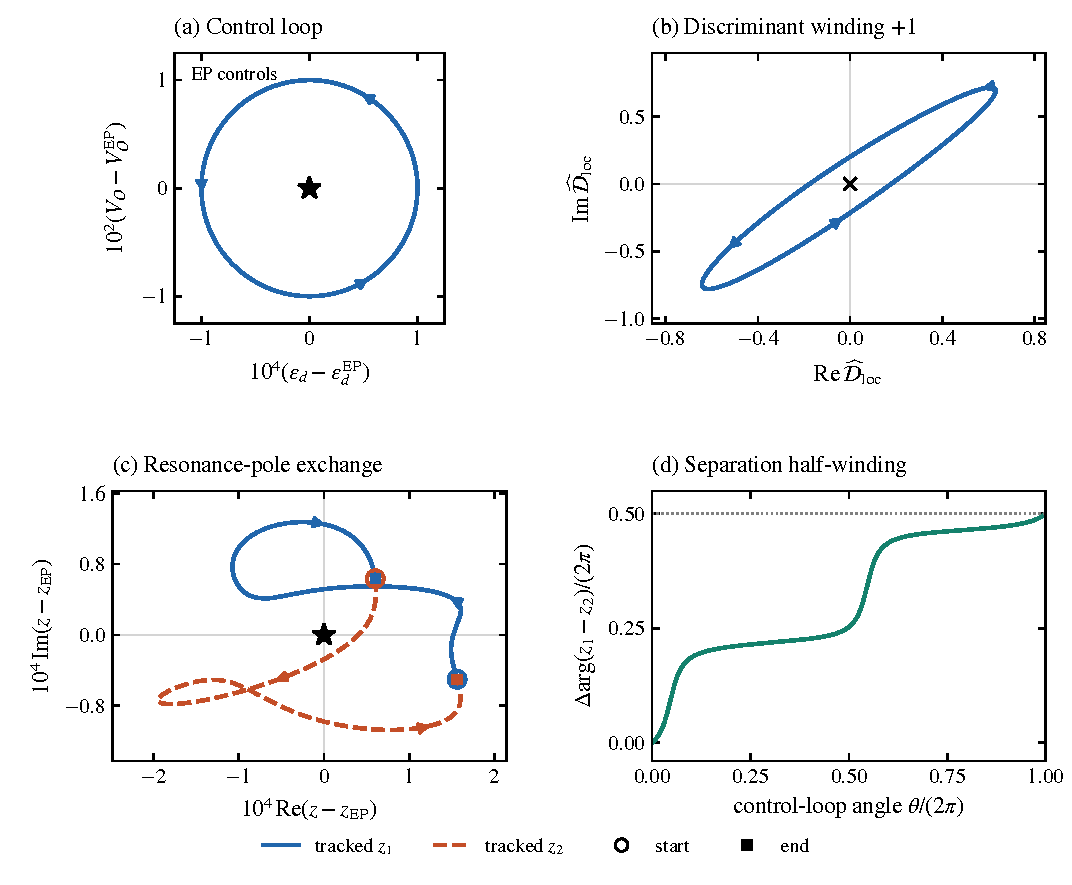
\includegraphics[width=0.88\textwidth]{SFig1_fullk_certificate.pdf}
\caption{%
\textbf{Full-momentum two-cut nonlinear causal-pole certificate.}
The stationary rotating-drive witness uses $\lambda=0.05$ and fixed $W=0.10$,
$K=\pi/4$, $\epsilon_O=120$, $\Omega=60$, and the solution in
Eq.~(\ref{eq:full_k_ep_solution}).
(a) The control ellipse encloses the EP controls; its half-widths are $10^{-4}$ in $\epsilon_d$ and $10^{-2}$ in $V_O$.
(b) $\hat{\cal D}_{\rm loc}={\cal D}_{\rm loc}/\max_C|{\cal D}_{\rm loc}|$
winds once around zero.
(c) Actual pole displacements from $z_{\rm EP}$ (star), with arrows showing
increasing control angle.  Open circles and filled squares mark the exact
initial and final points; the colours exchange at each endpoint.  These
curves are pole trajectories, not bath branch cuts, and need not individually
enclose the star.
(d) The continuously unwrapped separation phase advances by $\pi$ in one
circuit, giving half-winding $+1/2$.  All pole solves pass the separation and
residual guards.  The certificate concerns the full curved kernel, not its
constant-core approximation.
}
\label{fig:full_k_certificate}
\end{figure}

\subsection{Parameter continuation and real-frequency diagnostic}
\label{sec:continuation}
Continuation in SOC, with $W$ held fixed at $0.10$ while the real gate and
the off-shell auxiliary vertex are retuned by the same double-zero equations,
gives a finite locus over $0.02\leq\lambda\leq0.1578$
(Fig.~\ref{fig:full_k_soc_family}).  Independent local-winding and
pole-exchange certificates pass at $\lambda=0.05$, $0.10$, and $0.15$.  The continued pole approaches an open-channel threshold near the upper
end while the rate matrix remains passive.  The endpoint is not classified;
approach of $\operatorname{Re}z_{\rm EP}$ to a real threshold alone does not
establish a complex branch-point collision.  The isolated parameter values quoted above are
therefore points on a one-parameter family of causal pole EPs in the full
curved kernel, as expected for a codimension-two condition.

\begin{figure}[!htbp]
\centering
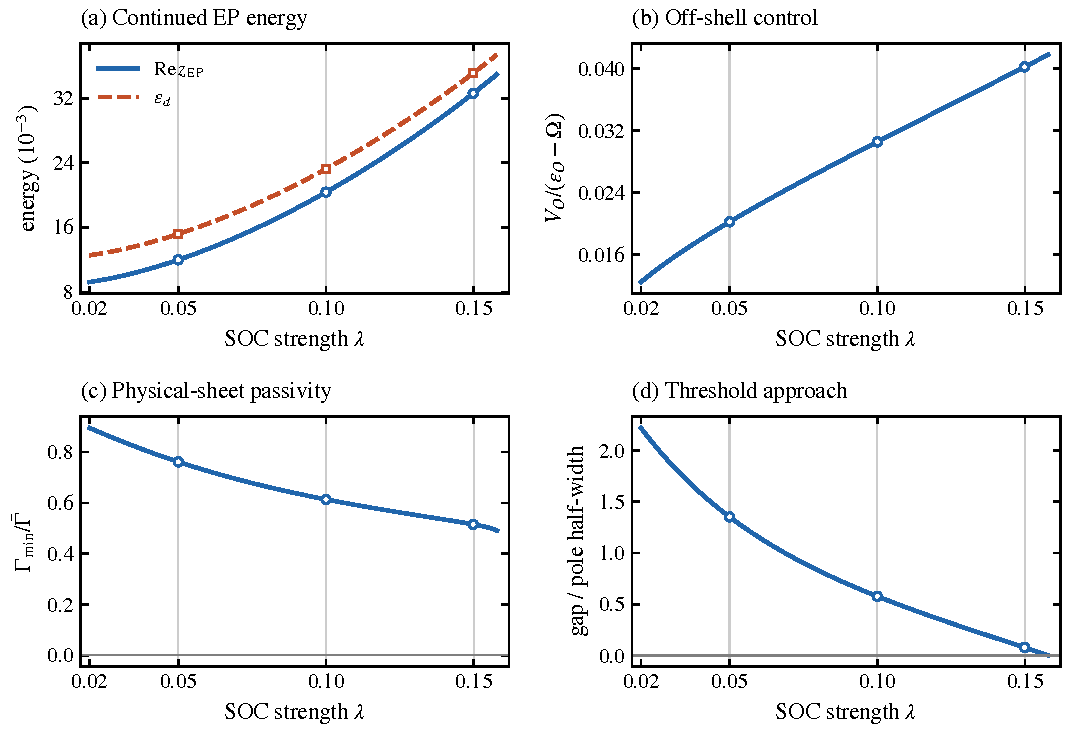
\includegraphics[width=0.94\textwidth]{Fig1_soc_family.pdf}
\caption{\textbf{SOC family of full-momentum nonlinear pole EPs.}
The double-zero equations are continued in $\lambda$ with $W=0.10$ fixed,
while the real impurity gate $\epsilon_d$ and the off-shell auxiliary vertex $V_O$ are retuned.  Vertical guides mark $\lambda=0.05$, $0.10$, and $0.15$,
where independent local-winding and pole-exchange certificates give winding
$+1$, pole permutation $(12)$, and half-winding $+1/2$.  The off-shell ratio
remains below $0.042$ and the physical rate matrix remains positive.  The
last panel shows the gap $(\operatorname{Re}z_{\rm EP}-\omega_{\rm th}^{+})/|\operatorname{Im}z_{\rm EP}|$
to the driven upper $k=0$ threshold.  This is
a one-dimensional locus in the enlarged parameter space; neither its
threshold endpoint nor a two-dimensional EP region is claimed.}
\label{fig:full_k_soc_family}
\end{figure}

Figure~\ref{fig:pt_phase} gives a complementary real-frequency diagnostic.
With $\epsilon_d$ and $V_O$ fixed at the $\lambda=0.10$, $\Omega=60$
certificate, choose the first scalar reference root $\omega_\ast$ of $\operatorname{Re}[\omega_\ast-\epsilon_d-\Sigma_0^R(\omega_\ast)]=0$
in the stated search window.  The retarded upper-rim self-energy defines
$s^2=\Sigma_x^2+\Sigma_z^2$, and the color shows
$C_s=\operatorname{Re}s^2/|s^2|$.  Positive and negative values indicate
predominantly real and imaginary frozen-matrix splitting, respectively.
Since $s^2$ is generally complex, the line $C_s=0$ is a crossover, not an
EP boundary or an exact $\PT$ transition.  Diagonalizing this kernel at
$\omega_\ast$ does not locate its complex resonance poles.  The marked EP
is independently obtained from $F=\partial_zF=0$.  As $\Omega$ varies,
$B_{\rm raw}(0)$ is subtracted anew: the slice holds the recentered bath
reference fixed, equivalent to adjusting the corresponding scalar bath
offset along with the drive.

\begin{figure}[htbp]
\centering
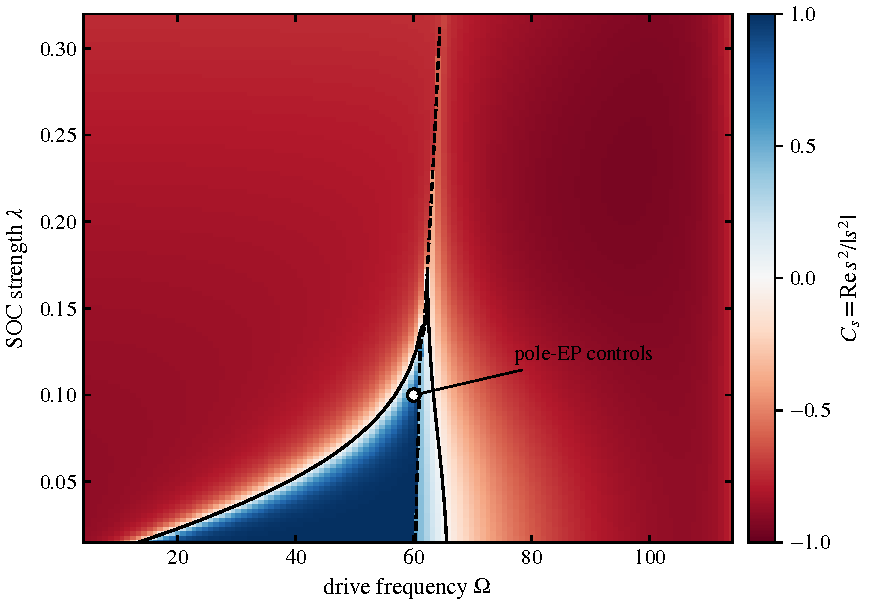
\includegraphics[width=0.62\textwidth]{Fig2_splitting_diagnostic.pdf}
\caption{\textbf{Retarded real-frequency splitting diagnostic.}
Color: $C_s=\operatorname{Re}(\Sigma_x^2+\Sigma_z^2)/|\Sigma_x^2+\Sigma_z^2|$
at the first scalar reference root $\omega_\ast\in(10^{-4},0.60)$.
The matrix is evaluated at $\omega_\ast+i\eta$, $\eta=10^{-10}>0$;
upper-rim convergence and positive half-widths are checked separately.
Parameters are $U=0$, $W=0.10$, $K=\pi/4$, $\epsilon_O=120$, $\epsilon_d=0.02323413$ and $V_O=1.83318448$.
Solid: $C_s=0$ crossover.  Dashed: change in the number of open channels
at $\omega_\ast$.  The circle marks controls of an independently certified
complex-pole EP.  Neither line defines a region of EPs or exact $\PT$ symmetry.}
\label{fig:pt_phase}
\end{figure}

\subsection{Finite-\texorpdfstring{$U$}{U} self-energy embedding}
\label{sec:finiteU}
We next test whether the representative \(\lambda=0.05\) causal pole EP
survives a local Anderson interaction without imposing the double-zero
condition on the interacting self-energy.  The positive \(2\times2\)
matrix spectral density of the same rotating full-\(k\) bath is logarithmically
discretized with \(\Lambda=1.5\), mapped by block Lanczos to a matrix Wilson
chain, and averaged over four \(z\) shifts.  We first use 12-site chains to
locate the finite-\(U\) center and evaluate
the zero-temperature correction-vector Green functions \(G\) and \(F\) in
exact fixed-charge sectors and form the equation-of-motion estimator (averaging the chain responses before taking
the matrix ratio)
\begin{equation}
\Sigma_U(z)=U F(z)G^{-1}(z).
\label{eq:finiteU_eom_selfenergy}
\end{equation}
Solving \(F_U=\partial_zF_U=0\) for the determinant of the full analytic
two-cut kernel dressed by Eq.~(\ref{eq:finiteU_eom_selfenergy}) gives, at
\(U=0.0025\),
\begin{equation}
\begin{split}
z_{\rm EP}^{(U)}&=0.01177670-0.00225815i,\\
\epsilon_d^{(U)}&=0.01440607,\qquad W^{(U)}=0.09036305.
\end{split}
\label{eq:finiteU_fullk_center}
\end{equation}
The complex poles belong to this approximate continuum-kernel embedding;
the closed Hermitian finite chain has real eigenvalues. Exact charge-sector
responses do not establish the continuum limit or the outgoing analytic
continuation of the interacting self-energy. These are separate from the
exact two-cut continuation of the noninteracting bath.
Here $U$ is $4\times10^{-3}$ of the bandwidth $\alpha_{\rm b}k_{\max}^2=0.617$,
while \(U/\bar\Gamma_{\rm self}=1.225\) with
\(\bar\Gamma_{\rm self}=(W^{(U)})^2/4=0.00204\).  The level lies about
$7\bar\Gamma_{\rm self}$ above the chemical potential, so the impurity is
nearly empty.  Direct $T=0$, $\mu=0$ checks on the same four-shift $N=12$
reference give $\langle n_d\rangle=0.017064$ and $\langle n_{d\uparrow}n_{d\downarrow}\rangle=5.73\times10^{-7}$
(Supplemental Material); the continuum saddle of Sec.~\ref{sec:finiteU_KR}
gives $0.024$ and $1.9\times10^{-6}$ at its own retuned EP.  The calculation
probes a weakly correlated impurity resonance and does not establish a
local-moment or Kondo regime.  Testing an occupied regime requires independent
pole retuning and bath-convergence checks; near-single occupancy and
suppressed double occupancy alone do not establish either an EP or Kondo
screening.  Section~\ref{sec:finiteU_KR} addresses both points with a saddle
that is evaluated on the continuum and on these chains. Additional occupied-bath tests find stable charge observables but
bath-dependent spin density and self-energy (SM App.~C); they do not
certify a continuum local-moment EP.

Figure~\ref{fig:finiteU_fullk_exact} gives the topological gate: on a small
control ellipse in $(\epsilon_d,W)$ the branch-tracked local discriminant has
winding $-1$, the two poles exchange, and all guards pass; $z$-average,
kept-space, and sum-rule checks are given in the Supplemental Material.  The
sign differs from the $U=0$ certificate because the degree depends on the
chosen pair of controls and its orientation; only its magnitude, one, is
fixed.

As an independent chain-length gate, the center is reoptimized separately
on the $N=10$ and $N=12$ complete-basis chains.  Their maximum relative
coordinate drift is $3.746\times10^{-3}$.  On a shared ellipse with
half-widths $2\times10^{-4}$ in $\epsilon_d$ and $2\times10^{-3}$ in $W$,
both chains have local-discriminant winding $-1$, endpoint pole exchange,
and pole-separation half-winding $-1/2$.  At 256 contour points,
\begin{equation}
\frac{\max_{j=1,\ldots,256}|D_{12,j}-D_{10,j}|}
{\min_{j=1,\ldots,256}|D_{10,j}|}
=\frac{1.638\times10^{-9}}{2.417\times10^{-9}}
=0.6775<1,
\label{eq:finiteU_fullk_rouche}
\end{equation}
which supports a nonvanishing straight-line homotopy on the resolved
contour.  A uniform version of this inequality, together with a smooth
critical-point branch over the enclosed domain, would preserve the Brouwer
degree.  The numerical maximum is not a bound between samples.  The
128-to-256 refinement and the independently tracked pole exchanges provide
finite-chain stability evidence, without bounding the omitted chain tail.

The two chain lengths hold one and two electrons in their ground states, so
the occupied part of the bath is represented coarsely.  At $U=0$ the 12-site
chains give $\langle n_d\rangle=0.0207$, against $0.0347$ for the continuum.
The $N=10\to12$ comparison therefore tests the topology but not this
occupied-bath resolution, and the coordinates in
Eq.~(\ref{eq:finiteU_fullk_center}) are specific to the chains;
Sec.~\ref{sec:finiteU_KR} compares them with a distinct continuum
mean-field approximation.

\begin{figure}[!htbp]
\centering
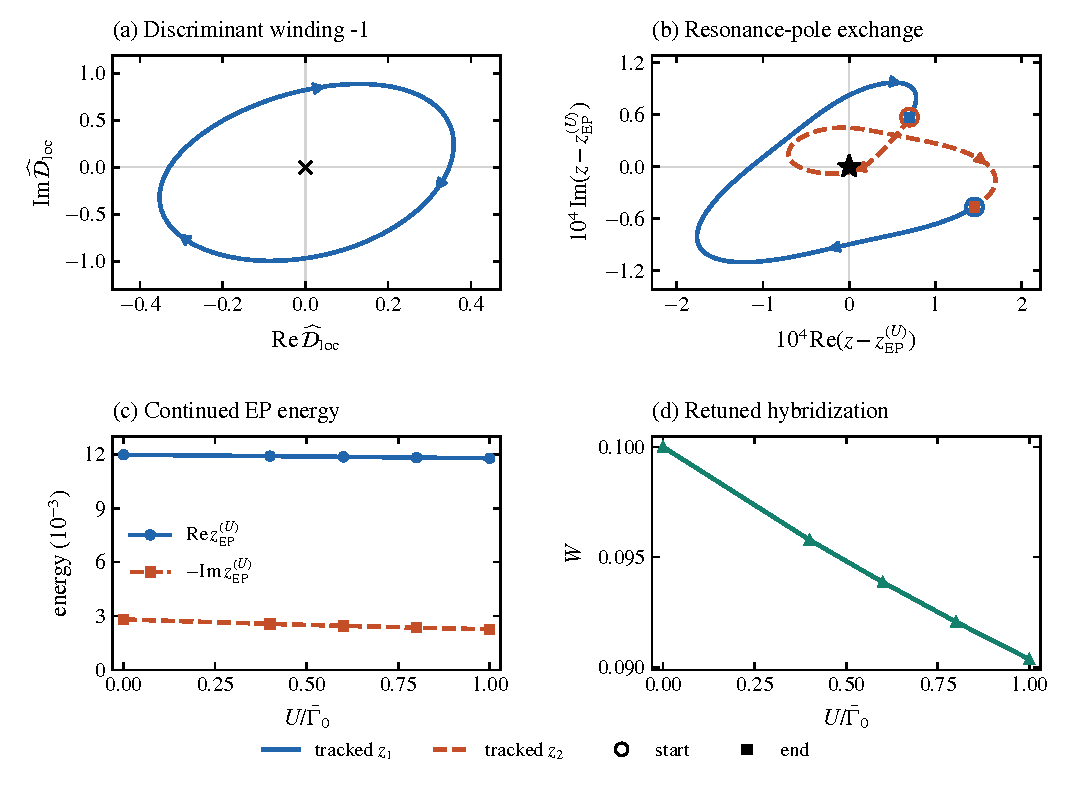
\includegraphics[width=0.98\textwidth]{Fig3_finiteU_fullk.pdf}
\caption{\textbf{Finite-\(U\) continuation of the causal full-\(k\) pole EP.}
(a) The branch-tracked local discriminant winds once clockwise around the
origin on the interacting control ellipse at \(U=0.0025\).
(b) The two nearby poles exchange after one circuit; open circles and filled
squares mark the initial and final tracked labels, and the star marks
Eq.~(\ref{eq:finiteU_fullk_center}).
(c) The center of the finite-chain self-energy embedding varies smoothly from \(U=0\) to
\(U/\bar\Gamma_0=1\), where \(\bar\Gamma_0=0.0025\).
(d) The retuned impurity hybridization $W$ on the same path.
The discriminant in (a) is normalized by its maximum modulus on the loop; the
displacement scale in (b) is $10^{-4}$.  Kept-space errors relative to the
exact response on the same four shifted 12-site chains are tabulated in SM
App.~C; they are not used to establish the winding.  The separate
$N=10\to12$ common-contour gate is
given by Eq.~(\ref{eq:finiteU_fullk_rouche}) and detailed in the Supplemental
Material.}
\label{fig:finiteU_fullk_exact}
\end{figure}

\begin{figure}[!htbp]
\centering
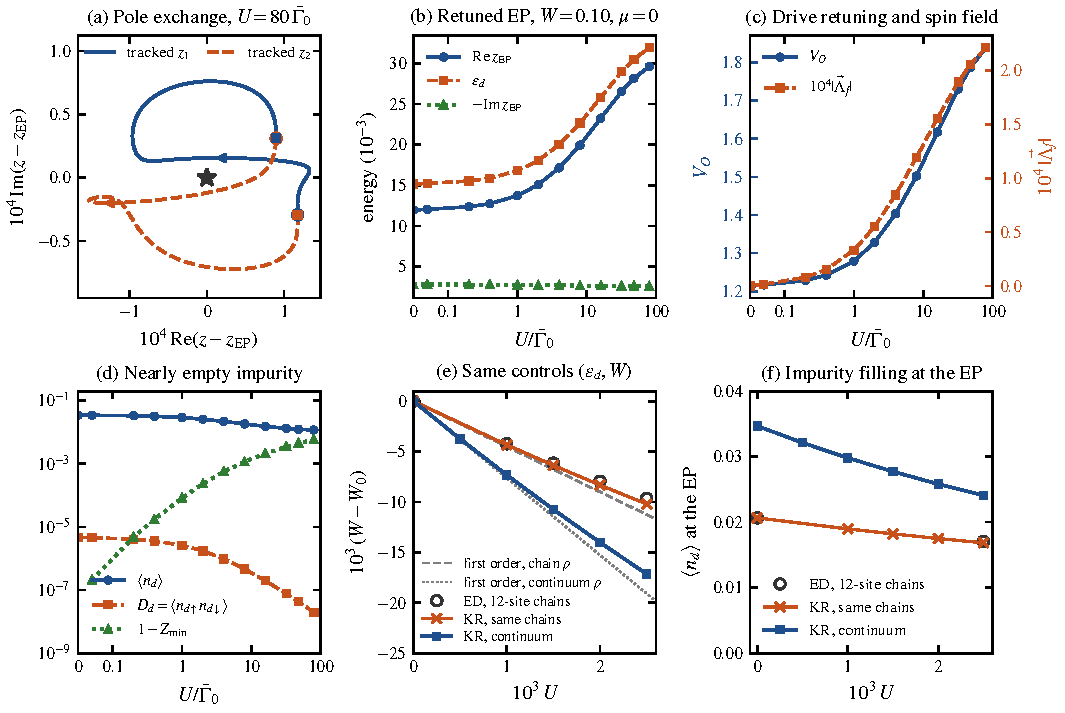
\includegraphics[width=0.98\textwidth]{Fig5_finiteU_KR.pdf}
\caption{\textbf{Finite-\(U\) continuation of the full-\(k\) resonance EP
with the continuum Kotliar--Ruckenstein saddle} ($T=0$).
(a) Pole exchange at $U=0.2=80\bar\Gamma_0$ ($\bar\Gamma_0=0.0025$, $\mu=0$)
on the control ellipse of Fig.~\ref{fig:full_k_certificate}, with the saddle
re-solved at each of 128 points.  Open circles and filled squares mark the
initial and final poles; the colours exchange at each endpoint, and the star
marks $z_{\rm EP}$.
(b) EP energy and gate on the branch with $W=0.10$ fixed and
$(\epsilon_d,V_O)$ retuned; $U=0$ is Eq.~(\ref{eq:full_k_ep_solution}).
(c) Retuned drive vertex and the traceless constraint field $|\vec\Lambda_f|$
that moves the EP.
(d) Impurity filling, double occupancy and smallest quasiparticle weight.
(e) Shift of $W$ for the controls of Sec.~\ref{sec:finiteU}, $(\epsilon_d,W)$
at fixed $V_O$: ED on the four 12-site chains (the path of
Eq.~(\ref{eq:finiteU_fullk_center})), KR with mesh-averaged inverse-kernel corrections on those chains, and
KR on the continuum.  Lines are the first-order Hartree--Fock
rates with the chain and continuum density matrices.
(f) Impurity filling at the EP for the same three calculations.
Panels (e,f) compare method and bath dependence; the different ED and KR
mesh averages are specified in SM App.~N.  All KR results are mean-field
saddle results.  The filling-one EP and its constrained continuation are
examined separately in Fig.~\ref{fig:KR_n1}.}
\label{fig:finiteU_KR}
\end{figure}

\subsection{Finite-\texorpdfstring{$U$}{U} continuation on the continuum bath}
\label{sec:finiteU_KR}

The finite-chain embedding establishes the numerical pole topology at the
tested chain sizes; convergence of the occupied bath remains unresolved.  To
separate bath discretization from the interaction approximation, we next use a
continuum-bath saddle.  The interaction enters the double-zero condition only through its self-energy near
the coalescing poles.  The spin-even part shifts both poles and is absorbed by
the gate, while the traceless part adds to the spin-odd and spin-mixing
channels of Eq.~(\ref{eq:full_k_pole_determinant}) and moves the double zero.
Because the $U=0$ EP has local degree $\pm1$ (Sec.~\ref{sec:causal_ep}), a
retuned EP persists, under the same smooth-branch assumption, while the
interaction keeps ${\cal D}_{\rm loc}\neq0$ on the certifying loop.  Globally,
this argument gives no protection once a discriminant zero crosses the loop,
or the smooth critical-point branch or chosen resonance sheet ceases to exist.
Interaction-induced changes of EP structure are possible~\cite{Schafer2022}.
At first
order in $U$ the self-energy is the static Hartree--Fock field
$\Sigma_{\rm HF}=U[(\operatorname{Tr}\rho)I-\rho]$, with $\rho_{\alpha\beta}=\langle d^\dagger_\beta d_\alpha\rangle=\rho_0I+\vec\rho\cdot\vec\sigma$.
Its traceless part $-U\vec\rho\cdot\vec\sigma$ is an exchange field along the
impurity polarization.  With the continuum $\rho$ of the $U=0$ witness it fixes
the initial retuning, $dW/dU=-7.63$ and $d\epsilon_d/dU=-0.551$ at fixed $V_O$.

Beyond first order we use the finite-$U$ Kotliar--Ruckenstein (KR)
slave-boson saddle~\cite{Kotliar1986} in its spin-rotation-covariant matrix
form~\cite{Lechermann2007}, at $T=0$ and with the preparation of
Sec.~\ref{sec:finiteU}.  A renormalization matrix $R$ and a real constraint
field $\Lambda_f=\Lambda_{f0}I+\vec\Lambda_f\cdot\vec\sigma$ enter the coherent
propagator $G_d(z)=R\,[zI-\Lambda_f-R\,\Sigma_d^{\rm II}(z)\,R]^{-1}R$.  The
bath kernel is integrated along the imaginary axis without discretization, and
$F_{\rm KR}=\det[zI-\Lambda_f-R\,\Sigma_d^{\rm II}R]=\partial_zF_{\rm KR}=0$ is
solved together with the saddle, which is re-solved whenever a control changes
(SM App.~N).  Since $R=I+O(U^2)$ and $\Lambda_f=\epsilon_dI+\Sigma_{\rm HF}+O(U^2)$,
the saddle reproduces the first-order self-energy; its retuning rates agree
with Hartree--Fock to better than 1\%. Quadrature refinement and independent functional derivatives support
numerical convergence within mean field; SM App.~N reports residuals,
local-stability checks and pole-loop refinement.



At $\mu=0$, with $W=0.10$ fixed and $(\epsilon_d,V_O)$ retuned
[Fig.~\ref{fig:finiteU_KR}(a)--(d)], the EP branch extends to
$U=0.2=80\bar\Gamma_0$ ($\bar\Gamma_0=0.0025$), or 0.32 of the bandwidth.
There $z_{\rm EP}=0.02963-0.00261i$, $\epsilon_d=0.03193$ and $V_O=1.8389$, with
both helicity channels open, positive rates and
$V_O/(\epsilon_O-\Omega)=0.031$; the retuning is of order one but saturates.
The impurity stays nearly empty, $\langle n_d\rangle=0.0118$ with $Z\geq0.994$,
while double occupancy is suppressed to $D_d=2.0\times10^{-8}$, $0.09$ of
$\det n$.  The EP is moved by the traceless field
$|\vec\Lambda_f|=2.2\times10^{-4}$, a third of the $U=0$ coherent coupling
$\operatorname{Re}\Sigma_z$.  At weak $U$ this field is the exchange part of
$\Sigma_{\rm HF}$; at strong $U$ it is a spin-dependent kinematic shift, the
level of one spin being pushed by the blocked hybridization of the other, a
mean-field counterpart of Haldane's level renormalization~\cite{Haldane1978}
in a polarized bath.  At $U/\bar\Gamma_0=8$ and 80 the loop of
Fig.~\ref{fig:full_k_certificate}, with the saddle re-solved at 128 points,
gives winding $+1$, pole exchange $(12)$ and half-winding $+1/2$
[Fig.~\ref{fig:finiteU_KR}(a)]; all three are unchanged at 256 intervals.

\begin{figure}[!htbp]
\centering
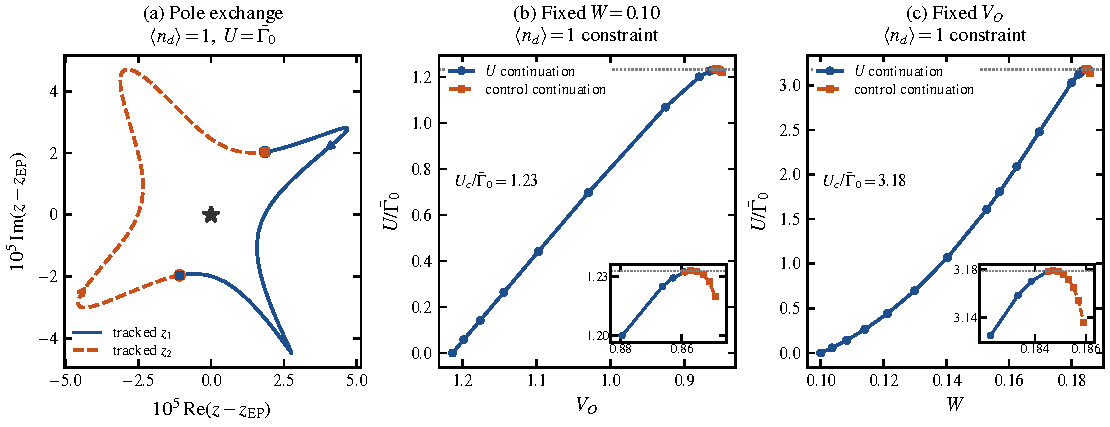
\includegraphics[width=0.98\textwidth]{Fig6_kr_filling_one.pdf}
\caption{\textbf{An occupied, charge-fluctuating EP and its constrained
continuation in the continuum KR saddle} ($T=0$).
(a) Pole exchange at $\langle n_d\rangle=1$ and $U=0.0025=\bar\Gamma_0$.
The star marks $z_{\rm EP}$; open circles and filled squares mark the
initial and final poles.  At the center, $D_d=0.229$ and $P_1=0.542$,
so this is not a local-moment state.  The loop keeps $\mu$ fixed and
re-solves the saddle; its controls and numerical checks are given in
SM App.~N.
(b,c) EP branches constrained to $\langle n_d\rangle=1$, with
$W=0.10$ or $V_O$ fixed, respectively.  Circles continue in $U$;
squares continue in the indicated control with $U$ as an unknown.
Insets resolve local folds at $U_c/\bar\Gamma_0=1.23$ and $3.18$.
Here $\bar\Gamma_0=0.0025$ is the fixed reference width, including in (c)
where $W$ varies.  These constrained turns do not exclude nearby EPs:
releasing the filling constraint yields the verified KR point
$U=0.0032$, $\langle n_d\rangle=0.98587$ (not plotted; SM App.~N).
All results are mean-field saddle results.}
\label{fig:KR_n1}
\end{figure}

Figure~\ref{fig:finiteU_KR}(e,f) compares ED and KR results on the
four 12-site chains with the continuum KR saddle.  The chain calculations
use different mesh averages: ED forms the self-energy from averaged
responses, whereas KR averages the individual inverse-kernel corrections
(SM App.~N).  Their shifts differ by 2.5--5.8\% in $W$ and 1.7--4.3\% in
$\epsilon_d$ over the tabulated interval.  These are observed differences,
not an isolated method-error bound.  The continuum KR shift of $W$ is
1.68--1.69 times its chain value, consistent with the chain's smaller
occupied density matrix.  The independently certified continuum KR point at
$U=0.0025$ has $W=0.082865$, $\epsilon_d=0.013902$ and
$z_{\rm EP}=0.011684-0.001874i$, with winding $-1$ and pole exchange.
No empirical correction of these coordinates is identified as an exact
continuum interacting result.





\subsection{Resonance EP at mean filling one}
\label{sec:KR_n1}

To test whether the mean-field EP is confined to a nearly empty impurity, we
also retune the chemical potential to obtain $\langle n_d\rangle=1$.
Figure~\ref{fig:KR_n1}(a) shows pole exchange at $U=0.0025=\bar\Gamma_0$,
with the saddle re-solved along the control loop.  At this EP,
$D_d=\langle n_{d\uparrow}n_{d\downarrow}\rangle=0.229$ against
$\det n=0.241$, and the single-occupancy probability is
$P_1=\langle n_d\rangle-2D_d=0.542$.  Thus mean filling one supports an EP
within the continuum KR approximation, but this state is charge fluctuating:
the mean occupation alone does not establish a local moment.

Keeping the filling exactly one gives local folds at
$U_c=0.003083$ when $(\epsilon_d,V_O,\mu)$ are retuned with $W=0.10$ fixed,
and $U_c=0.007948$ when $(\epsilon_d,W,\mu)$ are retuned with $V_O$ fixed
[Fig.~\ref{fig:KR_n1}(b,c)].  These are turns of constrained EP branches,
not boundaries of an EP-free phase.  Fixing $\mu$ at the first fold and
releasing the exact-filling constraint gives a locally stable EP at $U=0.0032>U_c$, $\langle n_d\rangle=0.98587$ and $D_d=0.21330$.
Its double-zero and rank-one checks, winding $-1$ and pole exchange are
reported in SM App.~N.  This nearby point demonstrates why the filling
constraint matters; with $P_1=0.55928$, it also remains charge fluctuating.

SM Fig.~S5 follows a separate occupied path without an EP search.  A
local-moment EP remains unresolved, motivating further work on
polarized-bath Kondo physics~\cite{Martinek2003NRG,Sindel2007}.



% ============================================================
\FloatBarrier
\section{Normalized Hamiltonian Benchmark and Emergent Non-Hermiticity}
\label{sec:Hss}
% ============================================================

\subsection{Projected Coefficients and Auxiliary Benchmark}
\label{sec:deriveHss}

At the slave-boson saddle (Sec.~\ref{sec:mf}), with gauge-invariant amplitude $r=|b_c|$, the impurity--bath vertex is $rW$.  Since an impurity self-energy
contains two spinon--bath vertices, the physical projected parametrization is $\Gpt=r^2\Gamma_{\rm PT}^{(0)}(\gb)$, $\Deff=r^2\Delta_0^{(0)}$ and $\Veff=rW$.
Here the superscript $(0)$ denotes the frozen bath projection before
slave-boson renormalization.  The core discriminant therefore carries a
common factor $r^4$, so the local core EP is exactly invariant under changes
of $r>0$ (Supplemental Material).  This invariance follows from a
renormalization common to both spins, as in the $U\to\infty$ saddle of
Sec.~\ref{sec:mf}; it does not protect the EP location.  A finite-$U$ saddle
gives spin-dependent quasiparticle factors and a traceless constraint field,
which move the EP (Sec.~\ref{sec:finiteU_KR}).
Supplemental Fig.~S1 uses $r=1$ and the normalized path $\Delta_{\rm eff}^{(0)}=0.50$, $\Gamma_{\rm PT}^{(0)}=|\beta_0|$; the scattering, saddle and flow checks use the archived fixed-$W$ path
$\Gamma_0=0.12$, $\Delta_{\rm eff}^{(0)}=0.075+0.050\beta_0$ and $\Gamma_{\rm PT}^{(0)}=0.20\beta_0$ (hence $\Delta_{\rm eff}^{(0)}=0.10$
at $\beta_0=0.50$).  The normalized geometry has symmetric crossings at
$\beta_0=\pm0.50$; the small-width audit uses only the positive window
$0.35\leq\beta_0\leq0.55$, with a crossing at $\beta_0=0.50$.

To display the constant-core geometry, we independently define a
four-component auxiliary benchmark at $\Dcoh=0$, in the basis
$(d_\uparrow,d_\downarrow,c_{k+},c_{k-})$.  Its local coefficients and
explicit two-level bath block are assigned independently; coefficients
already obtained by eliminating the physical bath must not be inserted
again together with that same bath.  This benchmark is not the physical
Dyson equation of Sec.~\ref{sec:coarse}:
\begin{equation}
\Hss(k)=
\begin{pmatrix}
\teps+i\Gpt & \Deff & \Veff/\sqrt{2} & \Veff/\sqrt{2}\\
\Deff & \teps-i\Gpt & \Veff/\sqrt{2} & -\Veff/\sqrt{2}\\
\Veff/\sqrt{2} & \Veff/\sqrt{2} & \varepsilon_{c,+}(k) & 0\\
\Veff/\sqrt{2} & -\Veff/\sqrt{2} & 0 & \varepsilon_{c,-}(k)
\end{pmatrix}.
\label{eq:Hss}
\end{equation}
Here $\teps=\epsilon_\xi+\delta_c+\dSig$ is the renormalized
impurity level.  The Lagrange multiplier $\delta_c$ enforces the
slave-boson constraint, while $\dSig$ is the real projected one-body
shift from the principal-value self-energy in Sec.~\ref{sec:PT_all}
(and may be absorbed into $\epsilon_\xi$ by convention).  The chiral
bath dispersions are $\varepsilon_{c,\pm}(k)=\alpha_{\rm b}k^2\pm\lambda k$.

For real coefficients, the antiunitary symmetry is $P_4\mathcal K$, with
$P_4=\operatorname{diag}(\sigma_x,1,-1)$ and complex conjugation $\mathcal K$;
the bath-channel sign is required to preserve the hybridization block.

\subsection{Diagonal-Hybridization Rotation}
\label{sec:rotation}

The hybridization block of $\Hss$ has Hadamard structure
$(\Veff/\sqrt{2})\bigl[\begin{smallmatrix}1&1\\1&-1
\end{smallmatrix}\bigr]$.
The unitary rotation
$U_2=\frac{1}{\sqrt{2}}\bigl[\begin{smallmatrix}
1&1\\1&-1\end{smallmatrix}\bigr]$
acting on the impurity subspace defines chiral spinon modes $\tilde{d}_\pm=(d_\uparrow\pm d_\downarrow)/\sqrt{2}$
and diagonalizes the hybridization block exactly.  In the
$(\tilde{d}_+,\tilde{d}_-,c_{k+},c_{k-})$ basis,
\begin{equation}
\Htilde(k)=
\begin{pmatrix}
\teps+\Deff & i\Gpt & \Veff & 0\\
i\Gpt & \teps-\Deff & 0 & \Veff\\
\Veff & 0 & \varepsilon_{c,+}(k) & 0\\
0 & \Veff & 0 & \varepsilon_{c,-}(k)
\end{pmatrix}.
\label{eq:Htilde}
\end{equation}
Here $\tilde d_+$ ($\tilde d_-$) hybridizes only with $c_{k+}$ ($c_{k-}$),
while the internal $i\Gpt$ term can still mix the two auxiliary
channels.  The frozen impurity eigenvalues are
$E_\pm=\teps\pm s$, $s=\sqrt{\Deff^2-\Gpt^2}$, on either path of
Sec.~\ref{sec:deriveHss}.  The plotted eigenvalues and condition numbers use the full
$4\times4$ kernel in Eq.~(\ref{eq:Htilde}).  Eliminating its bath block gives
\begin{equation}
\mathcal P(z,k)=\mathfrak p_+(z,k)\mathfrak p_-(z,k)+\Gpt^2=0,
\label{eq:full4_schur}
\end{equation}
where $\mathfrak p_\eta(z,k)=z-\teps-\eta\Deff-\Veff^2/[z-\varepsilon_{c,\eta}(k)]$ for $\eta=\pm$.
The full quadratic-kernel EP condition is $\mathcal P(z_{\rm EP},k)=\partial_z\mathcal P(z_{\rm EP},k)=0$.
At $k=0$ the bath energies coincide, so with
$\zeta(z)=z-\teps-\Veff^2/z$ this reduces to $\mathcal P(z,0)=\zeta(z)^2-\left(\Deff^2-\Gpt^2\right)$.
Thus the impurity-related double root occurs at $\Deff^2=\Gpt^2$ in this
common-shift limit; SOC-resolved finite-$k$ asymmetry generally unfolds it.
The declared nonzero-$k$ scan finds no additional interior EP because every
minimizer lies at its upper boundary.
This factorization concerns the auxiliary benchmark.  Its individual
eigenvalues are not identified with the full continuum resonance poles,
which are obtained from Eq.~(\ref{eq:full_k_pole_determinant}).

% ============================================================
\section{Slave-Boson Mean Field and Keldysh Self-Consistency}
\label{sec:mf}
% ============================================================

The effective impurity problem originates from a correlated Anderson
level with local repulsion $U$.  We formulate the constrained low-energy
sector using the $U\to\infty$ large-$N$ slave-boson mean-field
saddle~\cite{coleman1984mixed,read1983solution,SBkeld}.
This section tests a separately defined passive Markov kernel.  It supplies
neither the finite-$U$ self-energy of Sec.~\ref{sec:finiteU} nor the
finite-$U$ saddle of the full curved bath in Sec.~\ref{sec:finiteU_KR}.
Because a single boson renormalizes both spins equally, this saddle only
relabels $W\to rW$ and $\epsilon_\xi\to\teps$: it changes which bare controls
realize a given mean-field EP when an admissible saddle exists.  This mapping does not guarantee a finite saddle at arbitrary parameters or an unchanged complex pole in the full frequency-dependent bath.

\subsection{Slave-Boson Representation}

To handle the Coulomb repulsion $U$ in the Keldysh framework,
we use the large-$N$ slave-boson (SBMF)
representation~\cite{coleman1984mixed,read1983solution,SBkeld}:
$d^\dagger_\sigma=f^\dagger_\sigma b$ with
$b^\dagger b+\sum_\sigma f^\dagger_\sigma f_\sigma=Q$.
Here $f_\sigma$ are spinons, $b$ is the slave boson, and $Q=1$ for spin $1/2$; only the gauge-invariant amplitude $r=|b_c|$ enters observables.

The renormalized level is $\teps=\epsilon_\xi+\delta_c+\dSig$ and the
gauge-invariant SBMF scale is $\tb=|\gb|r$.
For the fixed-$W$ small-width path a seed-independent finite-$r$ solution exists at $T_{\rm b}=10^{-6}$ ($r\simeq0.0082$ at the core point; at $T_{\rm b}=0$ the saddle closes
analytically, and $r^2\Gamma_0$ equals the core-free scale $T_K^{(0)}$
at the core EP in the stated wide-band asymptotic, Supplemental Material), whereas at $T_{\rm b}=0.1$ the closure has no finite-$r$ branch, so the displayed spectra use frozen values (Supplemental Material).

\subsection{Saddle-Point Equations and Gauge-Invariant Amplitude}

Varying the complete contour action with respect to $\delta_c$ gives the
constraint $r^2+n_f=Q$.  In the integrated-bath representation, variation
with respect to $r$ gives the coherent-channel and complete influence-kernel
forces.  An explicit-bath hybridization force is an alternative description,
not an additional term for that same bath (Supplemental Material).

The resulting resonance reference is $\omega_{\rm res}\simeq{\rm Re}\,\teps$ (Supplemental Material).

\subsection{Near-EP screening-scale estimate}
The conventional Schrieffer--Wolff estimate in Eq.~(\ref{eq:TK_SW_est}) uses
positive real charge gaps and the bath density.  No biorthogonal-projector
residue enters its exponent; the supporting scale and flow checks are
given in the Supplemental Material.

% ============================================================
\section{Spectral Properties and Physical Regimes}
\label{sec:spectra}
% ============================================================

Supplemental Fig.~S1 displays the
dynamical fingerprints of the exact compensated core [panels (a)--(c)] and of
the relative gain--loss-only diagnostic limit [panels (d)--(f)].
The representative coefficients place a symmetric local EP pair at $|\gb|=0.5$,
accompanied by a condition-number peak and by a change from bounded
oscillation to growth of the dominant mode in the compensated representation.
Removing the coherent splitting channel [$\Deff=0$, panels (d)--(f)]
removes the coherent local impurity EP mechanism.  The remaining
relative gain--loss dynamics is retained only as a diagnostic contrast:
it should not be interpreted as a separate positive-screening Kondo
scale enhancement.

Condition numbers use the right-eigenvector matrix of the full $4\times4$ kernel with one normalization throughout and serve only to locate eigenvector coalescence.

\subsection{Causal Spectral Concentration and Weak-Flow Control}

The complete causal channel density and the channel-resolved weak-coupling
flow provide supporting tests of the analytic construction; the full panels
and adverse controls are shown in Supplemental Figs.~S2 and S3.  For $\beta_0=0.50$, the active/control ratios are $1.0567$ at $g_\ast=0.30$,
$1.0179$ at $g_\ast=0.40$, $0.9893$ at $g_\ast=0.50$, and $0.9166$ at
$g_\ast=1$.  In this flow the channel density is the impurity-resolved causal
density $(2\pi)^{-1}G^R\Gamma G^A$, not the bath spin density at the impurity
site; because the bare exchange is proportional to the identity, all EP
dependence of these ratios enters through that density.  They are therefore a
bounded diagnostic of the impurity resolvent in the stated window and do not
support an enhanced asymptotic Kondo temperature.

% ============================================================
\section{Fluctuation-Dissipation Relation and Spectral Functions}
\label{sec:FDR}
% ============================================================

For the supporting Keldysh calculation we assume a common thermal reservoir
distribution, $\Sigma^<=if\Gamma$, with consistent preparation of the
quadratic effective problem.  Stationarity of the rotating-frame Hamiltonian
alone does not establish this state assumption.  Under this closure, the
physical lesser Green's function is fixed by the bath self-energy.  The Supplemental Material verifies
that the impurity and bath fluctuation--dissipation relation (FDR) ratios
follow the same thermal Fermi function on spectral support, with maximum
residual $5.61\times10^{-14}$.  This is a consistency check of the specified closure, not a proof of driven thermalization.  No
mode-by-mode occupation of the non-Hermitian eigenvectors is used in the
physical FDR, in the occupations, or in the saddle-point equations.

The physical lesser function is the bath sandwich $G^<_{\rm phys}=G^R\Sigma^<_{\rm bath}G^A=f(G^A-G^R)$, which also satisfies number continuity, and the physical impurity DOS is $\rho_{\rm imp}=-\pi^{-1}{\rm Im\,Tr}[P_{\rm imp}G^R]\geq0$ (Supplemental Material).  A signed response of the relative kernel is not a DOS.

% ============================================================
\section{Real-Time Dynamics}
\label{sec:dynamics}
% ============================================================

The real-time diagnostic is the complex survival amplitude $O(t)=\langle \tilde d_+|e^{-i\Htilde t}|\tilde d_+\rangle$,
evaluated for the frozen kernel of Supplemental Fig.~S1(c),(f).
For the isolated two-component core, the eigenvalue separation is $2s$;
the coupled four-component benchmark also has bath-hybridization beating.
A defective block produces a $te^{-iE_{\rm EP}t}$ Jordan transient, while a
mode with positive imaginary eigenvalue grows in the compensated
representation.  With $\Deff=0$ [Supplemental Fig.~S1(d)--(f)] the isolated
block is broken for every $\Gpt\neq0$, so the coherent and relative-decay
channels are both needed for the core EP.

% ============================================================
\section{Causal Scattering and Linearized Contact Algebra}
\label{sec:scattering}
\label{sec:BA}
% ============================================================

\subsection{Complete scattering and Jordan response}

We use the standard Fisher--Lee and Wigner--Smith constructions
only as causal scattering diagnostics of the projected kernel
~\cite{fisherlee1981,wigner1955,smith1960}; they are not introduced here as
new formalisms.  For the compensated Markov kernel with positive rate matrix $\Gamma=2(\bar\Gamma I-\Gamma_{\rm PT}\sigma_z)$, the Fisher--Lee matrix $S=I-i\Gamma^{1/2}G^R\Gamma^{1/2}$ is unitary in the passive window and the Wigner--Smith matrix $Q=-iS^\dagger\partial_\omega S$ is Hermitian; only basis-invariant quantities (eigenphases, ${\rm Tr}\,Q$) are used (Supplemental Material).

For the compensated unbroken Markov core,
$s=\sqrt{\Delta_{\rm eff}^2-\Gamma_{\rm PT}^2}\in\mathbb R$ and the
two causal scattering phases give
\begin{align}
\operatorname{Tr}Q(\teps)
&=\frac{4\bar\Gamma}{s^2+\bar\Gamma^2},\nonumber\\
\frac{\operatorname{Tr}Q_{\Gamma_{\rm PT}}(\teps)}
{\operatorname{Tr}Q_{0}(\teps)}
&=\frac{\Delta_{\rm eff}^2+\bar\Gamma^2}
{\Delta_{\rm eff}^2-\Gamma_{\rm PT}^2+\bar\Gamma^2}>1 .
\label{eq:Smith_preep_ratio_main}
\end{align}
Thus, at fixed $\Delta_{\rm eff}$ and $\bar\Gamma$, the invariant scattering
phase density is analytically concentrated at the resonance center as the
EP is approached.  Its integrated weight remains fixed, and linewidth- or
rate-matched adverse controls need not share the peak ordering.  We call
Eq.~(\ref{eq:Smith_preep_ratio_main}) path-specific spectral concentration,
not an enhanced thermodynamic Kondo temperature or a basis-independent
amplification factor.

The cancellation responsible for its regularity is an exact matrix identity.
For the traceless core
$h=\Delta_{\rm eff}\sigma_x+i\Gamma_{\rm PT}\sigma_z$, $h^2=s^2I$, write
$a=z-\epsilon_0-\Sigma_0^R(z)$.  Although the individual biorthogonal
projectors $P_\pm=(I\pm h/s)/2$ grow as $1/s$, their complete resolvent is
\begin{equation}
G^R(z)=\frac{P_+}{a-s}+\frac{P_-}{a+s}
=\frac{aI+h}{a^2-s^2}.
\label{eq:complete_resolvent}
\end{equation}
At the EP, $h_{\rm EP}^2=0$, and $(aI-h_{\rm EP})^{-1} =\frac{I}{a}+\frac{h_{\rm EP}}{a^2}$,
so the coalescence produces a finite-coefficient simple-plus-double-pole
Jordan response, with no additional $1/s$ normalization multiplier.  This
cancellation is proved by Eq.~(\ref{eq:complete_resolvent}); it is not inferred
from NRG.  The separate NRG audit tests the nilpotent residue direction in a
spin-invariant, scalar-hybridization control. An exact interacting dimer
calculation establishes a nonzero double pole for that restricted control
(Supplemental Material); it does not establish protection in the driven
SOC bath. The full-bath interaction results are in Secs.~\ref{sec:finiteU} and~\ref{sec:finiteU_KR}.  At the EP ${\rm Tr}\,Q$ is a Lorentzian with $\int d\omega\,{\rm Tr}\,Q/(2\pi)=2$ whose center value $4/\bar\Gamma$ equals that of the Hermitian degeneracy.  An off-EP control with the same total rate has a larger raw proper-delay peak because one of its poles is slower; normalized by the slowest pole half-width, the largest proper delay at the EP is $1.83$ and $1.72$ times that of the Hermitian and off-EP controls (Supplemental Material).  The proper delay is therefore a coalescence fingerprint, not a Kondo-scale enhancement.

The same cancellation occurs in the finite-$U$ virtual-charge sum.  At
particle--hole symmetry, with $A=U/2$ and a channel-independent bare vertex $W$,
\begin{align}
J_{\rm SW}(s)
&=2W^2\left[(AI-h)^{-1}+(AI+h)^{-1}\right]
\notag\\
&=\frac{4AW^2}{A^2-s^2}I,\qquad
J_{\rm SW}(0)=\frac{8W^2}{U}.
\label{eq:SW_complete_charge}
\end{align}
Thus these complete core and virtual-charge expressions contain no
additional Petermann or condition-number multiplier.

\subsection{Low-energy contact-algebra and screening scope}
\label{sec:frozen_ba_main}

The eigenvalues $\mathsf{s}_a=e^{2i\delta_a}$ of the complete unitary
scattering matrix give the exact one-particle finite-size condition and phase
density
\begin{equation}
\det[I-e^{ik\mathcal L}S(k)]=0,
\qquad
\frac{1}{2\pi i}\partial_\omega\ln\det S
=\frac{1}{2\pi}\operatorname{Tr}Q .
\label{eq:contact_phase_compact}
\end{equation}
After equal-velocity branchwise linearization with a constant component matrix and scalar hybridization, the finite-$U$ two-electron contact matrix is the rational Anderson $R$ matrix in a dressed rapidity; it obeys the Yang--Baxter equation, is $GL(2,\mathbb C)$ covariant, and the corresponding finite-ring boundary problem admits a unipotent
twist, with transformed contact terms and operator domain retained
(Supplemental Material and Ref.~\cite{KulkarniYB2026}).  No full-momentum integrability is claimed.

For comparison with the causal weak-flow calculation, the only screening
estimate retained is the conventional frozen Schrieffer--Wolff form
\begin{equation}
\begin{aligned}
J_a^{\rm SW}&=2|W_a|^2
\left(\Delta_{0,a}^{-1}+\Delta_{2,a}^{-1}\right),\\
T_{K,a}^{\rm SW(est)}&\simeq D_{{\rm uv},a}
\exp[-1/(\chi_K\rho_{b,a}J_a^{\rm SW})].
\end{aligned}
\label{eq:TK_SW_est}
\end{equation}
Here $\Delta_{0,a},\Delta_{2,a}>0$ are real empty- and double-charge excitation
costs in a conventional local-moment reference and $\rho_{b,a}$ is its bath
density.  The coefficient $\chi_K$ is defined by the one-loop convention
$dj/d\ell=\chi_Kj^2$, with $j=\rho_bJ$ and
$\ell=\ln(D_{\rm uv}/\Lambda_{\rm run})$ for running cutoff
$\Lambda_{\rm run}$.  This estimate is not evaluated at the nearly empty EP
witness and does not replace a complex charge denominator by its modulus.

% ============================================================

% ============================================================
\section{Conclusions}
\label{sec:conc}
% ============================================================

The stationary rotating drive controls a family of resonance EPs in the
defined finite-band radial SOC impurity model. In the constant-vertex,
two-open-channel window it supplies coherent spin-odd coupling and
modifies the SOC-induced relative decay. The full-frequency double zero,
rank-one kernel and pole exchange establish the coalescence numerically
while the physical decay rates remain positive. This is the principal
result: the microscopic controls reach an EP of the causal resonance
problem beyond its normalized constant-core approximation.

The interaction calculations probe continuation of that result. The
finite-chain self-energy embedding retains the tested topology at $N=10$
and $12$, without establishing convergence of the occupied bath. The
continuum KR approximation extends the low-filling EP to
$U=80\bar\Gamma_0$ and admits charge-fluctuating EPs at and near mean
filling one. Nearby EPs persist beyond folds of the exactly filling-one
branches. A local-moment EP and exact thermodynamic interaction survival
remain unresolved.

The supporting analyses delimit the interpretation. Complete propagators
and the restricted virtual-charge sum cancel divergent individual
projectors; the normalized proper delay does not establish enhanced Kondo
screening. The scalar-bath Jordan control and equal-velocity contact
algebra concern separately specified models. Their symmetry restrictions
cannot be imposed on the full SOC self-energy to infer an interacting EP. The next interaction test is a continuum-converged
self-energy at an occupied, charge-quenched point, followed by retuning
the resonance pair. Pumped screening additionally requires specified
reservoirs and consistent retarded and lesser self-energies.

\section*{Code and data availability}
The original certificates and finite-chain outputs are archived in
Release v2.1.0, \href{https://doi.org/10.5281/zenodo.21888925}{doi:10.5281/zenodo.21888925},
and the public repository
\href{https://github.com/VMKPHYSMATH/emergent-pt-dirac-impurity}{\nolinkurl{VMKPHYSMATH/emergent-pt-dirac-impurity}}~\cite{kulkarni2026code}.
The revision of 28 October 2026 provides the corrected manuscript,
finite-$U$ saddles, filling and bath-convergence checks, supporting symmetry
control, validation records and figure sources in the repository's
\href{https://github.com/VMKPHYSMATH/emergent-pt-dirac-impurity/tree/revision/stationary-drive-20261028/revisions/20261028}{dated revision directory}.
This revision is distinct from v2.1.0. A matching fixed-version GitHub
release and Zenodo deposit will be completed before journal submission;
their identifiers will be added after deposition.
The all-versions record is
\href{https://doi.org/10.5281/zenodo.21434682}{doi:10.5281/zenodo.21434682}.

\begin{acknowledgments}
This work was carried out independently.

The author thanks Rok \v{Z}itko for helpful discussions on NRG methodology
and continuum convergence, and colleagues and workshop participants for
discussions on driven quantum impurity systems, non-Hermitian many-body
physics, and Keldysh methods.
OpenAI's ChatGPT (Codex) assisted with editing, code, figures and
numerical and algebraic checks. Anthropic's Claude assisted with the
finite-$U$ saddle checks, figures and editing. The author is responsible
for the scientific content.
\end{acknowledgments}

\nocite{ChaoPalacios2011,KawakamiOkiji1982,Wiegmann1980,WiegmannTsvelick1983,anderson1970poor}
% Flush REVTeX bibliography controls before its legacy end-document hook.
% This preserves longbibliography/article titles with newer LaTeX kernels.
\makeatletter
\write@bibliographystyle
\makeatother
\bibliography{ref}

% Restore natbib's end-of-document consistency check under the bundled REVTeX.
\makeatletter
\NAT@swatrue\let\bibcite\NAT@testdef
\makeatother
\end{document}
